\subsubsection{ReportBuilder - reporty biznesowe}
	\textbf{ReportBuilder} jest narzędziem będącym obecnie w fazie rozwoju, niemniej pozwalającym już teraz na tworzenie raportów biznesowych. Dedykowany dla użytkownika, daje mu możliwość wybrania zbioru interesujących go tabel, kolumn które zebrane razem stanowią logiczny zbiór używany w dalszej kolejności do konstrukcji zapytania do bazy danych i utworzenia gotowego raportu. Nie udało się znaleźć żadnego rozwiązania, które można by wykorzystać bezpośrednio w aplikacji WEB. Przewodnik składa się z 4 wymaganych kroków:
	\begin{enumerate}
		\item wybranie tabeli, dla której wygenerowany zostanie raport
		\item dostosowanie formatowania kolumn,
		\item podanie danych opisujących raport: tytuł, podtytuł, opis.
	\end{enumerate}		
	
	\begin{figure}[H]
		\centering
		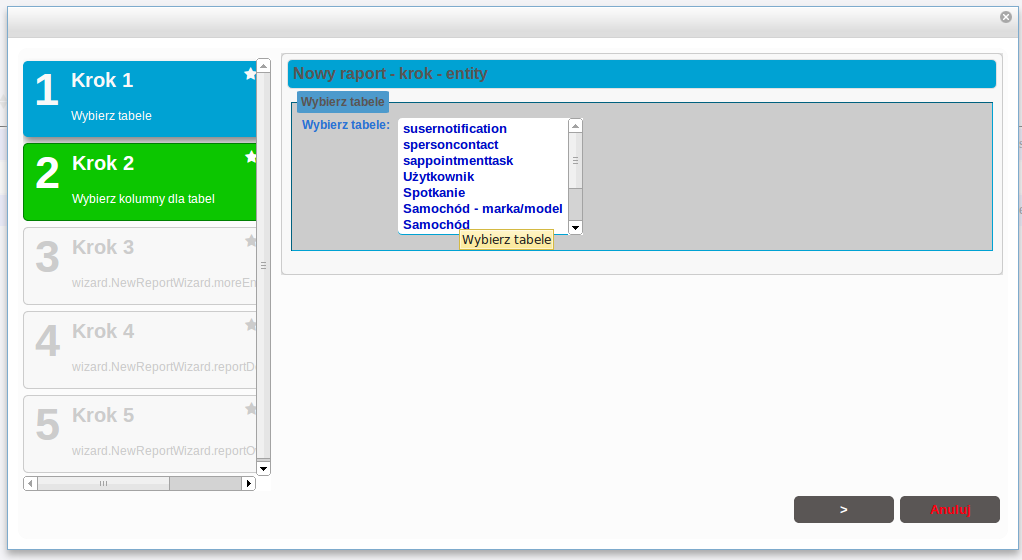
\includegraphics[width=1.0\textwidth]{images/rbuilder_step1}
		\caption[Kreator nowego raportu - krok 1]{
			Kreator nowego raportu - krok 1
		}
		\label{app:wizard_newReport_step1}
	\end{figure}	
	\begin{figure}[H]
		\centering
		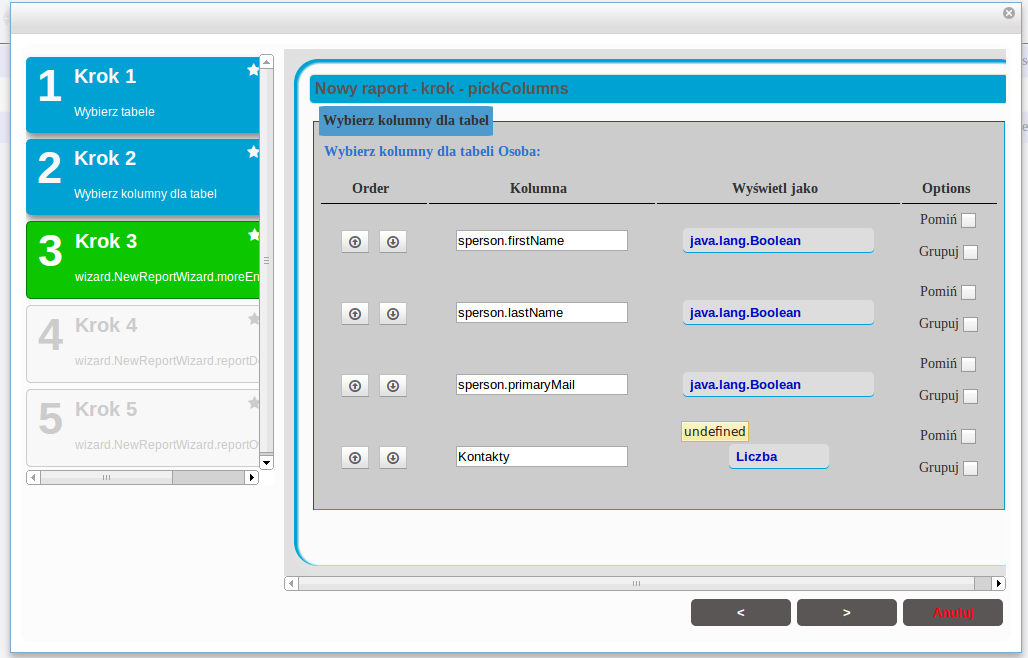
\includegraphics[width=1.0\textwidth]{images/rbuilder_step2}
		\caption[Kreator nowego raportu - krok 2]{
			Kreator nowego raportu - krok 2
		}
		\label{app:wizard_newReport_step2}
	\end{figure}		
	\begin{figure}[H]
		\centering
		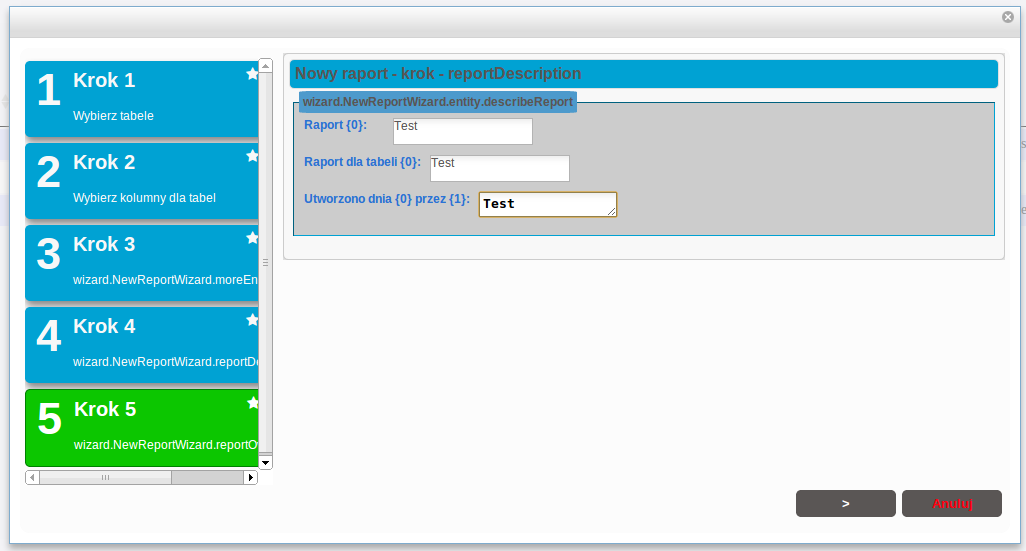
\includegraphics[width=1.0\textwidth]{images/rbuilder_step3}
		\caption[Kreator nowego raportu - krok 3]{
			Kreator nowego raportu - krok 3
		}
		\label{app:wizard_newReport_step2}
	\end{figure}	
	
	\begin{wrapfigure}{r}{0.5\textwidth}
		\centering
		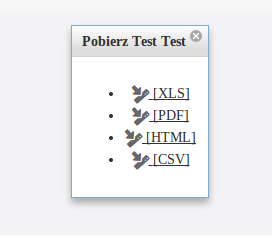
\includegraphics[width=1.0\textwidth]{images/rbuilder_generateReport}
		\caption[Generowanie nowego raportu - wybór docelowego formatu]{
			Generowanie nowego raportu - wybór docelowego formatu: \textbf{PDF}, \textbf{XLS}, \textbf{CSV}, \textbf{HTML}
		}
		\vspace{-10pt}
		\label{app:wizard_newReport_generateReport}
	\end{wrapfigure}
	
	Dzięki możliwości wykonywania akcji na poszczególnych wierszach tabeli, udało się przypisać dla każdego raportu link uruchamiający jego
	generowania oraz usunięcie. Usunięcie jest operacją trywialną z punktu widzenia użytkownika, ponieważ nie widzi on niczego poza 
	końcowym rezultatem. Z drugiej strony w momencie kliknięcia na przycisk \textbf{Generuj}, użytkownik ma możliwość
	wybrania końcowego formatu w jakim chciałby zobaczyć swoje dane. 
	Dalsza część funkcjonalności, czyli faktycznego zrenderowania gotowych danych została zaimplementowana z użyciem biblioteki wspierającej
	\textbf{JasperReports}, pochodzącą ze szkieletu aplikacji \textbf{Spring}. Przykładowy raport wygląda w następujący sposób:
	\begin{figure}[H]
		\centering
		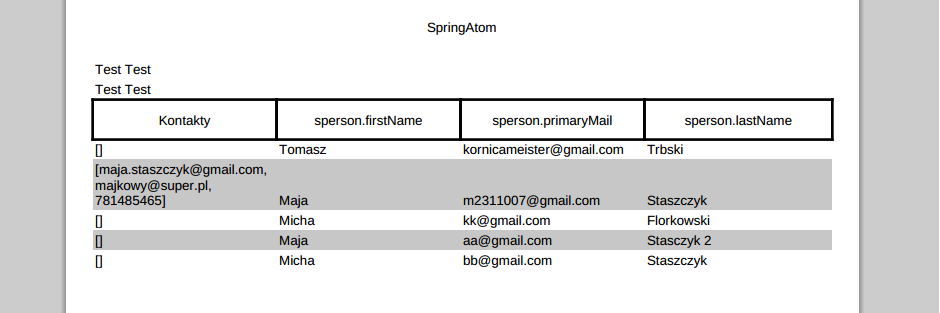
\includegraphics[width=1.0\textwidth]{images/rbuilder_report}
		\caption[Gotowy raport utworzony przez komponent \textbf{RBuilder}]{
			Gotowy raport utworzony przez komponent \textbf{RBuilder}
		}
		\label{app:wizard_newReport_report}
	\end{figure}		

\pagebreak
\subsubsection{Kreator nowego użytkownika}
	Kreator nowego użytkownika pozwala na tworzenie nowy obiektów klasy \textbf{SUser}. Kwestia uprawnień jest tutaj szczególnie ważna z uwagi na to, że w przewodniku wybierany jest zestaw ról. Role, do których przypisany jest użytkownik, stanowią późniejszą bazę do weryfikacji dostępności funkcji systemu dla poszczególnych użytkowników. 
	\begin{figure}[H]
		\centering
		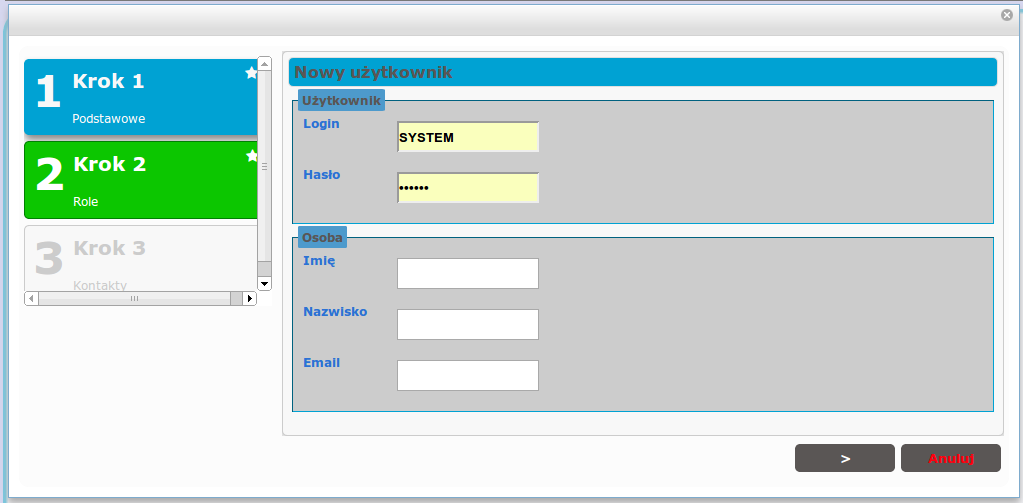
\includegraphics[width=1.0\textwidth]{images/newUser-basic}
		\caption[Kreator nowego użytkownika - dane podstawowe]{
			Kreator nowego użytkownika - dane podstawowe	
		}
		\label{app:newUser_basic}
	\end{figure}	
	\begin{figure}[H]
		\centering
		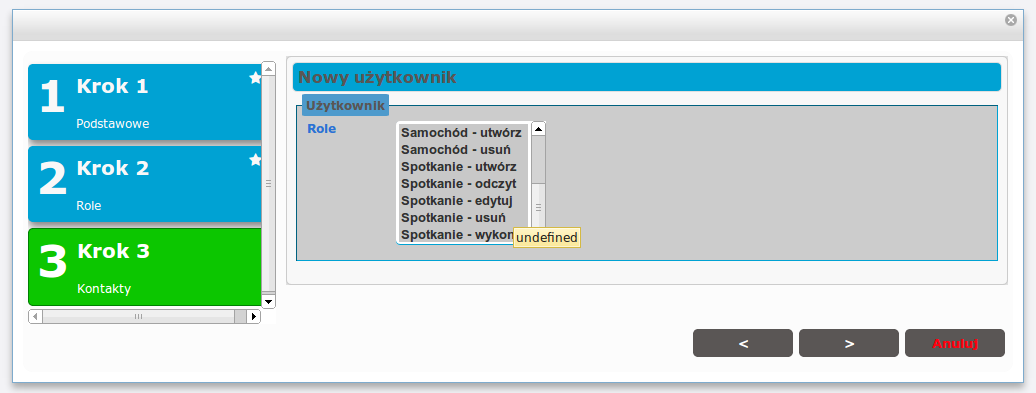
\includegraphics[width=1.0\textwidth]{images/newUser-roles}
		\caption[Kreator nowego użytkownika - uprawnienia użytkownika]{
			Kreator nowego użytkownika - uprawnienia użytkownika
		}
		\label{app:newUser_roles}
	\end{figure}	
	\begin{figure}[H]
		\centering
		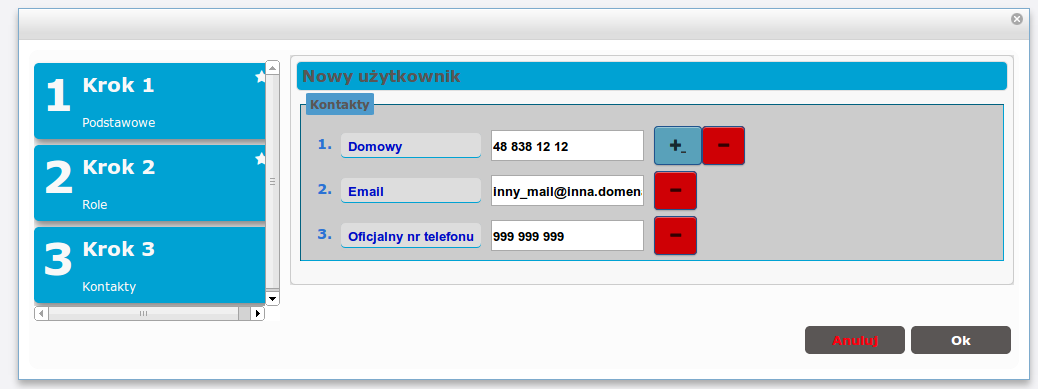
\includegraphics[width=1.0\textwidth]{images/newUser-contacts}
		\caption[Kreator nowego użytkownika - dane kontaktowe]{
			Kreator nowego użytkownika - dane kontaktowe
		}
		\label{app:newUser_contacts}
	\end{figure}	

\subsubsection{Kreator nowego samochodu}
	Kreator nowego samochodu został zaprojektowany aby tworzyć nowe obiekty klasy \textbf{SCar}.	Pierwszym krokiem jest podanie \textbf{numeru VIN}, z którego system odczytuje wszelkie możliwe dane, które można odkodować korzystając z informacji dostępnych publicznie. Na obecną chwilę są to:
	\begin{itemize}
		\item rok produkcji, zwracany jako lista lat w których samochód mógł być wyprodukowany,
		\item kraj, w którym samochód został wyprodukowany.
	\end{itemize}
	
	W drugim kroku kreator nowego samochodu podaje takie informacje jak:
	\begin{itemize}
		\item markę oraz model,
		\item numer tablicy rejestracyjnej,
		\item rok produkcji,
		\item rodzaj paliwa,
		\item właściciela.
	\end{itemize}
	\begin{figure}[H]
		\centering
		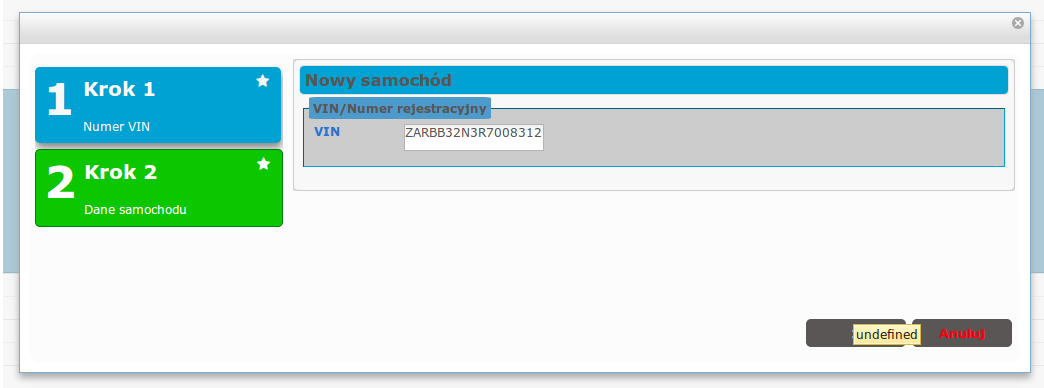
\includegraphics[width=1.0\textwidth]{images/newCar-vin}
		\caption[Kreator nowego samochodu - numer VIN]{
			Kreator nowego samochodu - numer VIN
		}
		\label{app:newCar_vin}
	\end{figure}	
	\begin{figure}[H]
		\centering
		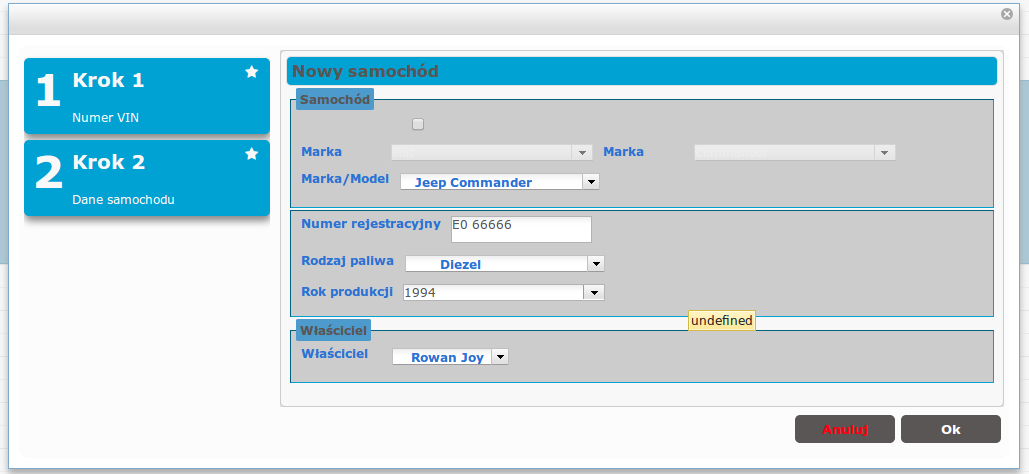
\includegraphics[width=1.0\textwidth]{images/newCar-data}
		\caption[Kreator nowego samochodu - pozostałe dane]{
			Kreator nowego samochodu - pozostałe dane
		}
		\label{app:newCar_data}
	\end{figure}

\subsubsection{Organizator spotkań}
	Organizator spotkań jest komponentem wspierającym zarządzania tym typem obiektów. 
	Pozwala na wgląd w listę wszystkich spotkań na 4 rożne sposoby:
	\begin{itemize}
		\item widok w kontekście wybranego dnia,
		\item widok w kontekście wybranego tygodnia,
		\item widok w kontekście wybranego miesiąca,
		\item widok tabelaryczny wszystkich spotkań.
	\end{itemize}
	
	\begin{figure}[H]
		\centering
		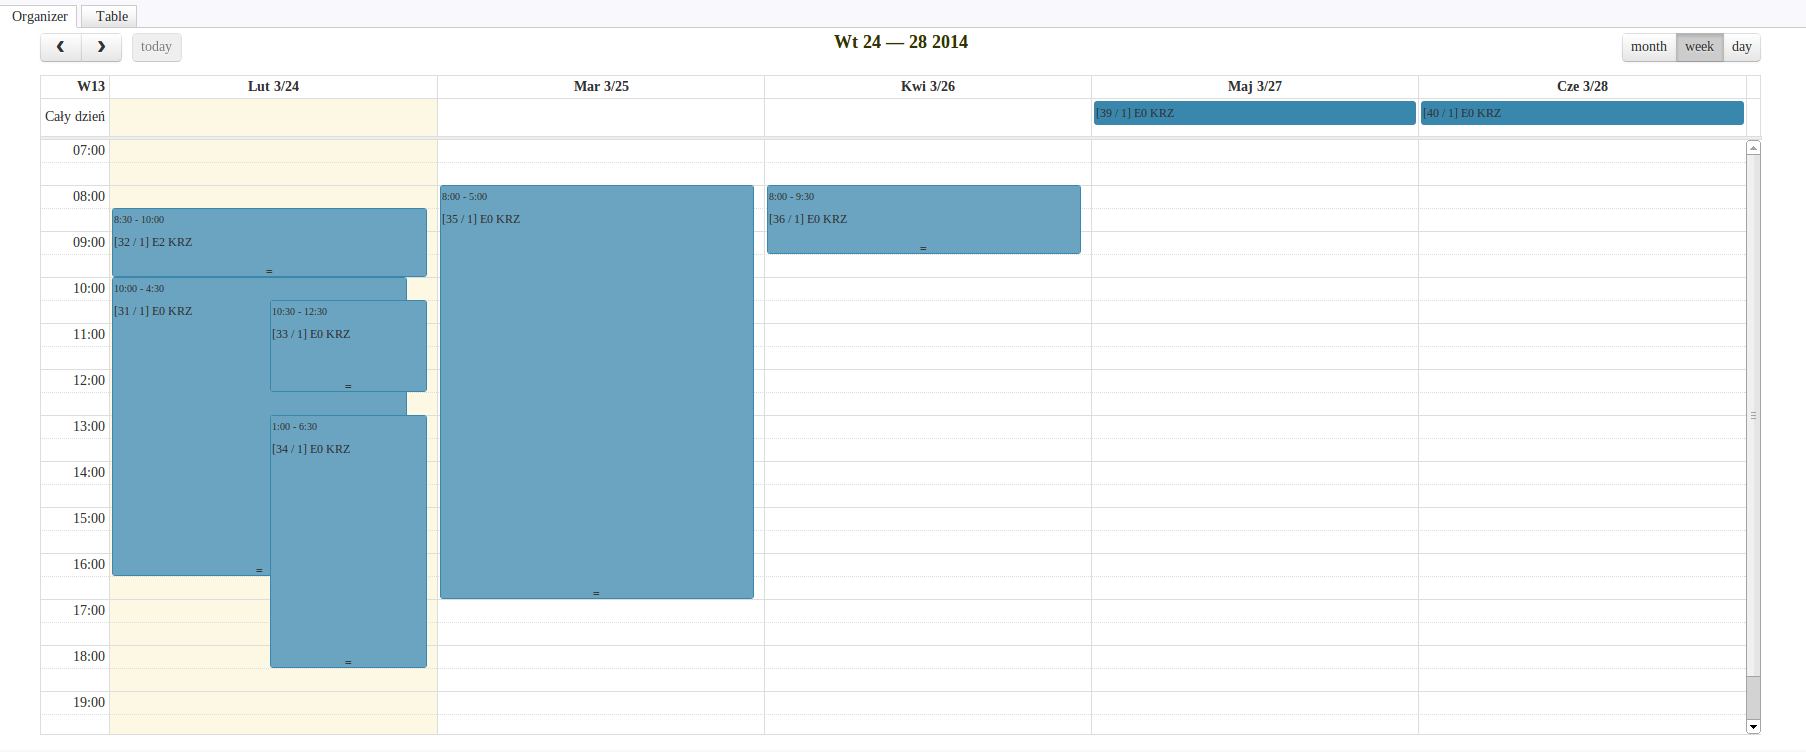
\includegraphics[width=1.0\textwidth]{images/calendarComponent-organizer}
		\caption[Komponent kalendarza wspierający organizację spotkań - organizer]{
			Komponent kalendarza wspierający organizację spotkań - organizer		
		}
		\label{app:component_calendar_organizer}
	\end{figure}	
	\begin{figure}[H]
		\centering
		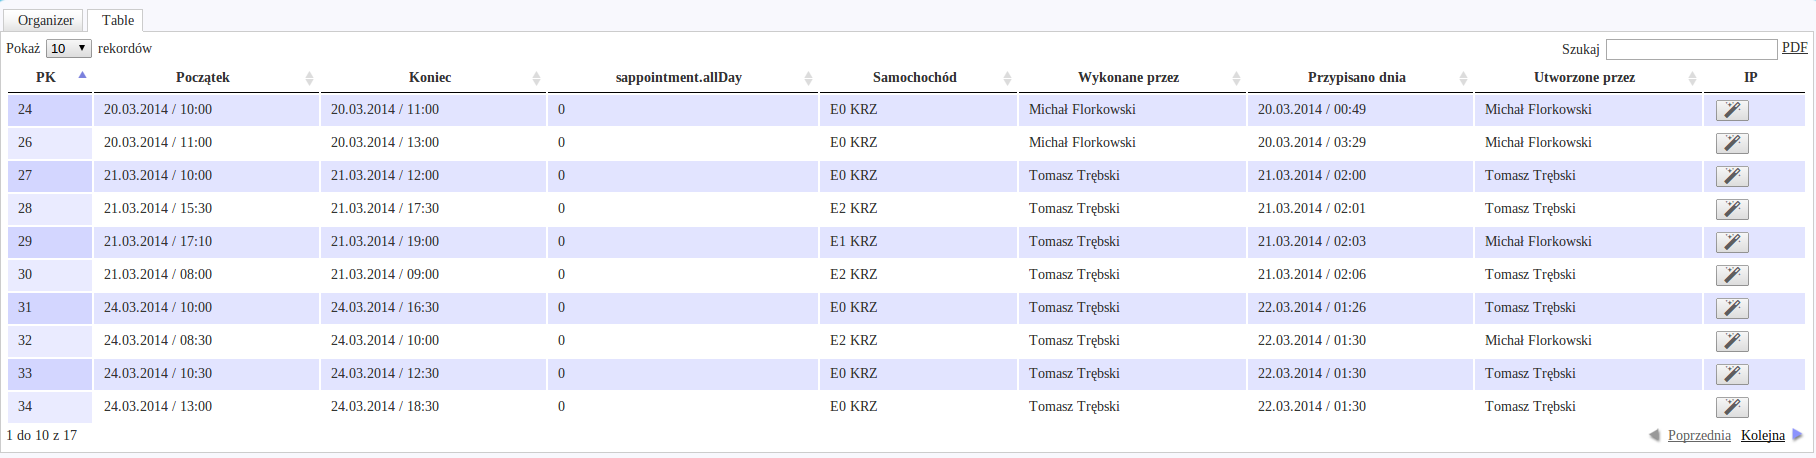
\includegraphics[width=1.0\textwidth]{images/calendarComponent-table}
		\caption[Komponent kalendarza wspierający organizację spotkań - tabela]{
			Komponent kalendarza wspierający organizację spotkań - tabela	
		}
		\label{app:component_calendar_table}
	\end{figure}	
	
	Z poziomu organizera możliwe jest natomiast otwarcie strony domenowej dla wybranego spotkania, dostarczającej znacznie więcej informacji niż sam organizator oraz uruchomienie przewodnika utworzenia nowego spotkania. Ważną cechą tego przewodnika jest to, że zakres dat wybrany w organizatorze jest zachowany. Sam kreator został napisany w oparciu o technologię \textbf{Spring Web Flow}, dzięki czemu na poziomie jednego komponentu można wprowadzić dane takie jak: 
	\begin{itemize}
		\item mechanik, który będzie odpowiedzialny za wizytę,
		\item mechanik raportujący dane spotkanie, niemniej taką możliwość posiadają jedynie osoby uprawnione do tego,
		\item wybrany samochód,
		\item lista zadań do wykonania podczas wizyty,
		\item opcjonalny komentarz dla wizyty.
	\end{itemize}
	
	\begin{figure}[H]
		\centering
		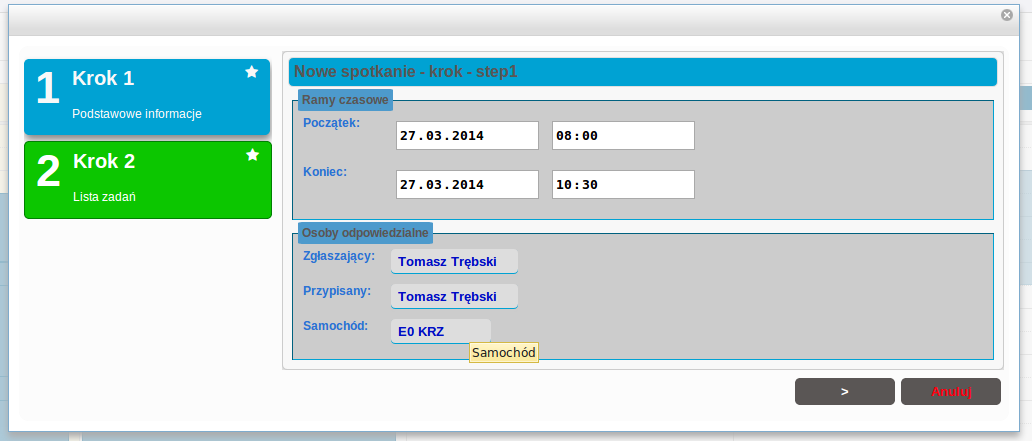
\includegraphics[width=1.0\textwidth]{images/newAppointment_step1}
		\caption[Kreator nowego spotkania - krok 1]{
			Kreator nowego spotkania - krok 1
		}
		\label{app:wizard_newAppointment_step1}
	\end{figure}
	\begin{figure}[H]
		\centering
		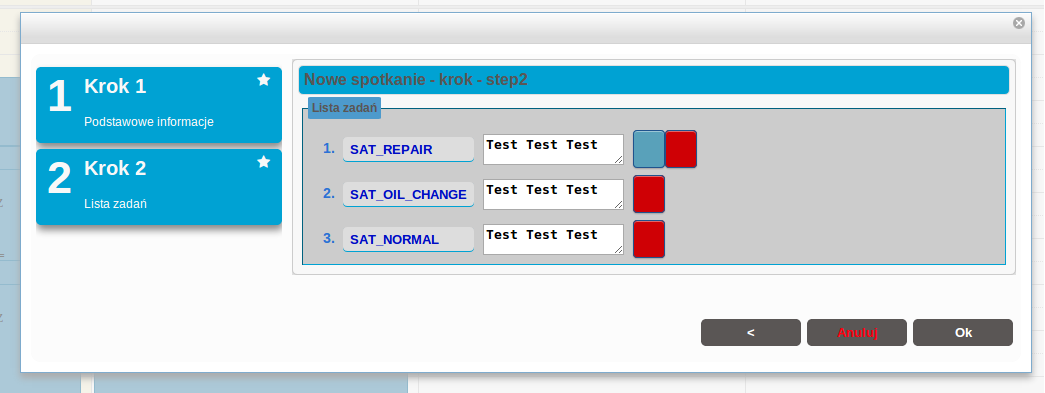
\includegraphics[width=1.0\textwidth]{images/newAppointment_step2}
		\caption[Kreator nowego spotkania - krok 2]{
			Kreator nowego spotkania - krok 2
		}
		\label{app:wizard_newAppointment_step2}
	\end{figure}
	\begin{figure}[H]
		\centering
		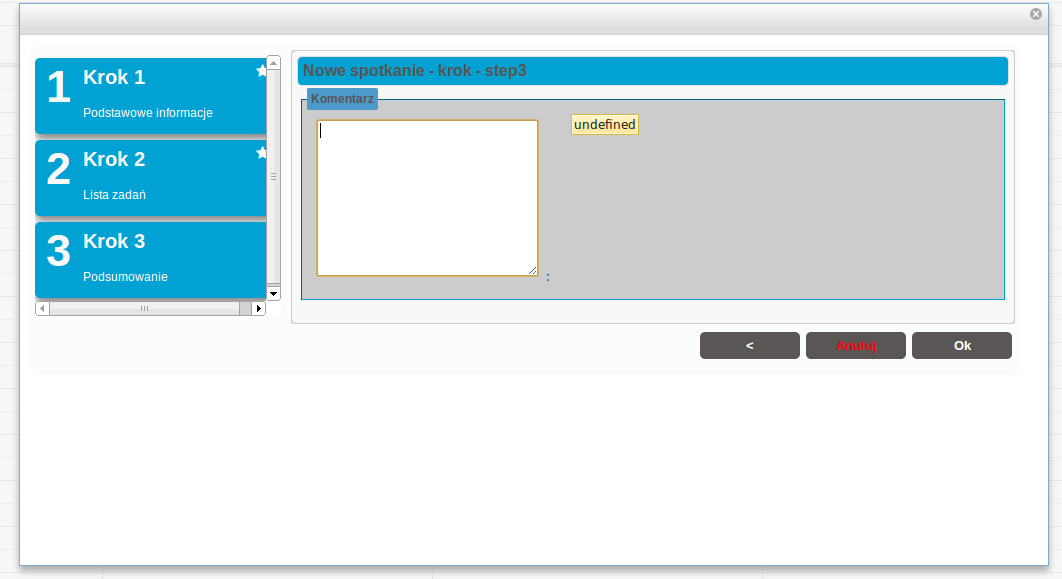
\includegraphics[width=1.0\textwidth]{images/newAppointment_step3}
		\caption[Kreator nowego spotkania - krok 3]{
			Kreator nowego spotkania - krok 3
		}
		\label{app:wizard_newAppointment_step3}
	\end{figure}		
	
	Dane wejściowe są walidowane pod kątem logiki biznesowej:
	\begin{itemize}
		\item termin spotkania:
		\begin{itemize}
			\item podane godziny (oraz czas) muszą mieścić się w wybranym zakresie [7-21],
			\item koniec spotkania nie może nastąpić później niż jego początek,
			\item zbyt krótkie (30 minut) oraz zbyt długie (10 dni),
			\item pokrywa się z co najmniej jednym spotkaniem dla mechanika wybranego jako wykonawca
		\end{itemize} 
		\item wybrany samochód:
		\begin{itemize}
			\item jeśli z właścicielem samochodu powiązane są jakiekolwiek problematyczne informacje, wyświetlane jest ostrzeżenie
		\end{itemize}
	\end{itemize}